\documentclass[letterpaper]{article}
\usepackage{amsmath}
\usepackage{tikz}
\usepackage{epigraph}
\usepackage{lipsum}
\usepackage{hyperref}
\usepackage{tocloft}
\usepackage{wrapfig}

\usepackage{setspace, amsmath}

\usepackage[centering,includeheadfoot,margin=2cm]{geometry}
\usepackage{xcolor}
\usepackage{calc,blindtext}

\renewcommand\epigraphflush{flushright}
\renewcommand\epigraphsize{\normalsize}
\setlength\epigraphwidth{0.6\textwidth}

\definecolor{titlepagecolor}{cmyk}{1,.60,0,.40}

\DeclareFixedFont{\titlefont}{T1}{ppl}{b}{it}{1.0in}

\def\printauthor{%
    {\large \@author}}
\makeatother
\author{%
    Nico Taljaard \\
    10153285 \\%vspace{20pt} \\
    Gerhard Smit \\
    12282945 \\%vspace{20pt} \\
    Martin Schoeman \\
    10651994 \\
}

\begin{document}

\begin{titlepage}

\newcommand{\HRule}{\rule{\linewidth}{0.5mm}} % Defines a new command for the horizontal lines, change thickness here

\begin{center} % Center everything on the page
 
%----------------------------------------------------------------------------------------
%   HEADING SECTIONS
%----------------------------------------------------------------------------------------

%\textsc{\LARGE University Name}\\[1.5cm] % Name of your university/college

\includegraphics[width=70mm]{laminin.png} \\
\textsc{\Large University of Pretoria}\\[0.2cm] % Major heading such as course name
\textsc{\large Derivco - Rodney Pillay}\\[0.2cm] % Minor heading such as course title

%----------------------------------------------------------------------------------------
%   TITLE SECTION
%----------------------------------------------------------------------------------------

\HRule \\[0.4cm]
{ \huge \bfseries Corpse Slasher by Laminin}\\[0.4cm] % Title of your document
\HRule \\[0.5cm]
 
%----------------------------------------------------------------------------------------
%   AUTHOR SECTION
%----------------------------------------------------------------------------------------

\begin{minipage}{0.4\textwidth}
\begin{flushleft} \large
\emph{COS 301 Software Engineering}\\
\vspace{1cm}\textbf{Project Management}
\end{flushleft}
\end{minipage}
~
\begin{minipage}{0.4\textwidth}
	\begin{flushright} \large
	\emph{Developers:} \\
		%\printauthor % Supervisor's Name
		NJ \textsc{Taljaard} \\
			\begin{small}
				10153285
			\end{small} \\
		M  \textsc{Schoeman} \\
			\begin{small}
				10651994 \\
			\end{small}
		G  \textsc{Smit} \\
			\begin{small}
				12282945
			\end{small}
	\end{flushright}
\end{minipage}\\

% If you don't want a supervisor, uncomment the two lines below and remove the section above
%\Large \emph{Author:}\\
%John \textsc{Smith}\\[3cm] % Your name

%----------------------------------------------------------------------------------------
%   LOGO SECTION
%----------------------------------------------------------------------------------------


\includegraphics[width=70mm, height=90mm]{corpseslasher.png}\\ % Include a department/university logo - this will require the graphicx package
 
%----------------------------------------------------------------------------------------
\end{center}
\vfill % Fill the rest of the page with whitespace

\end{titlepage}
	\newpage
	{\LARGE \bf Change Log}\\[2em]
	
	\begin{tabbing}
		\hspace*{2.5cm}\=\hspace*{2.5cm}\=\hspace*{8cm}\=\hspace*{3cm} \kill
		13/10/2014	\> Version 1.0	\> Document Created.							\> Gerhard Smit \\
		13/10/2014	\> Version 1.0	\> Development process \& team portfolio. 		\> Nico Taljaard \\
		14/10/2014	\> Version 1.0	\> Issue management \& project status.			\> Nico Taljaard \\
		14/10/2014	\> Version 1.0	\> Unimplemented functionality.					\> Nico Taljaard \\
		14/10/2014	\> Version 1.0	\> Risk \& challenges. 							\> Nico Taljaard \\
		
		
	\end{tabbing}
	
		\newpage
		\renewcommand\contentsname{TABLE OF CONTENTS}
		\newcommand\contentsnameLC{\colorbox{black}{\makebox[\textwidth-2\fboxsep][l]{\bfseries\color{red} Table of Contents}}}
		
		\renewcommand{\cftdot}{}
		\hypersetup{linktocpage}
		\tableofcontents
		
		\begin{flushleft}
			\LARGE\href{https://github.com/njTaljaard/Laminin_CorpseSlasher/}{Git repository: Laminin\_CorpseSlasher}
		\end{flushleft}
		
	\newpage
	\section*{\colorbox{black}{\makebox[\textwidth-2\fboxsep][l]{\bfseries\color{red} Software development process }}} \addcontentsline{toc}{section}{Software development process}
		\vspace{0.1in}
		
		\begin{huge}
			\textbf{Scrum}
		\end{huge}
		to allow for agile movement and changes to the system but to retain a concrete process methodology to aim to complete our milestone \& complete the project ideally. This gave use the freedom to self-organize our team responsibilities and with the help of our Project Owner prioritize our project milestones and functionality. \\ \\
		\textbf{Project roles:}
		\begin{itemize}
			\item Project Owner \\
					Rodney Pillay from Derivco is assigned as our project owner as a mentor, approval of created user stories, educate stakeholders on the development process, to negotiate priorities scope, funding \& most of all milestone reviews.
			\item Development Team \\
					Nico Taljaard, Martin Schoeman, Gerhard Smit - Responsible for development of the final product but also to have a potential shippable version at all times. This was achieved by have a working version as master, enabling lower brunches for implementation, changes \& re-factoring.
			\item Scrum Master \\
					Nico Taljaard has responsibility of communication between development team and project owner as chair in meetings, challenge \& coordinates team.  \\
		\end{itemize}
		
		\noindent\textbf{Sprints:} \\
		Sprints were created on a biweekly bases to maintain progress throughout the project and to ensure that milestone deadlines where met. Milestone as well as corresponding issues is created on git so that all stakeholders and the development team can follow project progress. \\
		
		\noindent\textbf{Meetings:}
		\begin{itemize}
			\item Sprint planning meetings \\
					Sprint cycles where made on a biweekly basis, planning what will be able to achieve before the next stakeholder meeting. Each development member would say what he will be able to complete, it is documented and the progress was tracked until each issue is completed. These meetings where held after our meeting with the project owner.
			\item Scrum meetings \\
					Is used to track the progress of each sprint task, which have been completed. If an issues occurs with a task it is documented and determined if it will be able to be completed, if the issue can not be resolved before the end of a sprint it is place in the backlog for the following sprint. This was held when we where on campus or over email/messaging.
			\item End meetings \\
					Were held on a biweekly basis with the project owner where he would review the complete work, progress of the project, problems or bugs in development, what went amiss during the sprint and what went right. Discusses are held about what to prioritize for the next sprint and if our the focus needs to be shifted to another part of the project.  \\
		\end{itemize}
		 
		\noindent\textbf{Backlogs:} \\
			Project and sprint backlog is managed on git through milestones and issues which will be discussed later in this document. \\
			
		\noindent\textbf{Spikes:} \\
			Spikes is extremely relevant during the progress of this project where we are working with unknown \& new technologies. This resulted in a lot of time spent in research, creating test cases to determine if it will work in regards to the project. The applicable technologies are the game engine itself, sub aspects of the engine, 3D modelling, rigging, animation, back-end system, OAuth for social media. \\
			
		\noindent\textbf{Sashimi:} \\
			At the start of the project before any development occurred we created our user stories to depict the project main aim \& what are the main completion goals are of the project to deliver a complete product at the end.
			
		\vspace{0.2in}
	\section*{\colorbox{black}{\makebox[\textwidth-2\fboxsep][l]{\bfseries\color{red} Team profile }}} \addcontentsline{toc}{section}{Team profile}
		\vspace{0.1in}
		
		\begin{Large} 
			\textbf{Nico Taljaard} - 10153285 \\
		\end{Large}
		
		\begin{minipage}[l]{0.23\textwidth}
			\begin{flushleft}
				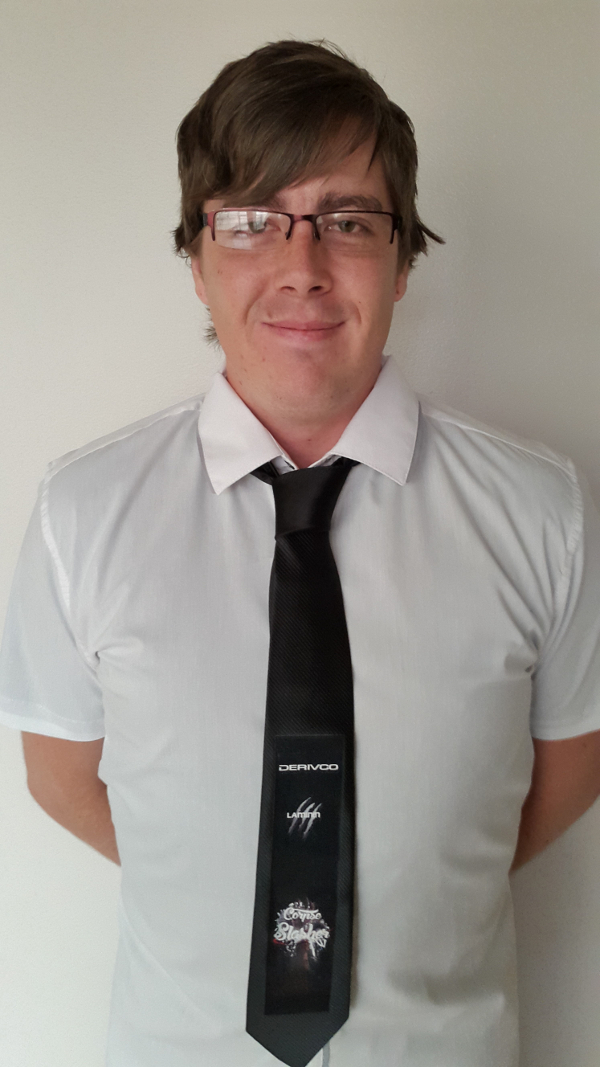
\includegraphics[width=30mm,height=50mm]{Members/Nico.jpg}
			\end{flushleft}
		\end{minipage}
		\begin{minipage}[r]{0.75\textwidth}
			\begin{itemize}
				\item Scrum Master.
				\item Work distribution \& coordination.
				\item Client communication control.
				\item Game design \& development.
				\item Model design, edit, rigging \& animation.
				\item Port of game to Android.
				\item Game non-functional testing.
				\item Documentation.
			\end{itemize}
		\end{minipage} \\ \\
		
		\begin{flushleft}
			\begin{Large}
				\textbf{Martin Schoeman} - 10651994 \\
			\end{Large}
		\end{flushleft}
		
		\begin{minipage}[l]{0.23\textwidth}
			\begin{flushleft}
				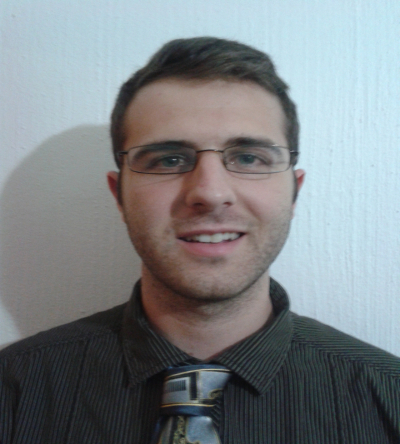
\includegraphics[width=30mm,height=50mm]{Members/Martin.jpg}
			\end{flushleft}
		\end{minipage}
		\begin{minipage}[r]{0.75\textwidth}
			\begin{itemize}
				\item Back-end development.
				\item Database implementation \& management.
				\item OAuth login and post implementation.
				\item Client side network implementation.
				\item Client server integration.
				\item Server unit testing.
				\item Documentation.
			\end{itemize}
		\end{minipage}
		
		\newpage
		\begin{flushleft}
			\begin{Large}
				\textbf{Gerhard Smit} - 12282945 \\
			\end{Large}
		\end{flushleft}
				
		\begin{minipage}[l]{0.23\textwidth}
			\begin{flushleft}
				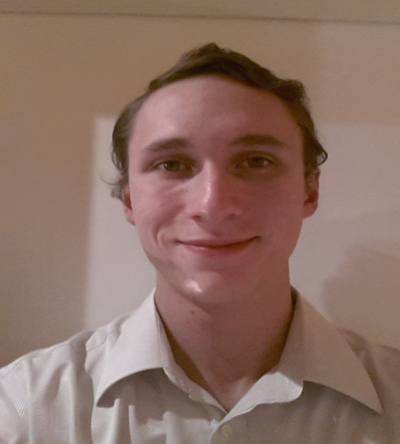
\includegraphics[width=30mm,height=50mm]{Members/Gerhard.jpg}
			\end{flushleft}
		\end{minipage}
		\begin{minipage}[r]{0.75\textwidth}
				\begin{itemize}
					\item User interface design and implementation.
					\item User interface controls \& settings to game.
					\item User interface port to Android.
					\item Game \& server integration.
					\item Documentation.
				\end{itemize}
		\end{minipage}
		
		\vspace{0.2in}
	\section*{\colorbox{black}{\makebox[\textwidth-2\fboxsep][l]{\bfseries\color{red} Issue management}}} \addcontentsline{toc}{section}{Issue management}
		\vspace{0.1in}
		
		We are using git as our version control which supports functionality for creating milestones \& issues that have been used throughout the project for tracking and control. Throughout the project we had a total of 337 commits to bring the project to what it is now.
			
		\begin{itemize}
			\item Milestones:
				\begin{itemize}
					\item 21 Milestone created.
					\item Overview break down of project.
					\item Main objective of project.
					\item Controlled due dates.
					\item Project progression reinforcement.
				\end{itemize}
			\item Issues:
				\begin{itemize}
					\item 153 Issues created.
					\item Detailed section of milestones.
					\item Sub-division of milestones for team assignment.
					\item Take of milestone progression.
					\item Log of assignments.
					\item Log of reported error.
				\end{itemize}
			\item Stakeholder Tracking:
				\begin{itemize}
					\item Overall project progress.
					\item Member contribution to tasks and project.
					\item Bug or errors that are being struggled with.
				\end{itemize}
		\end{itemize}
		
		\vspace{0.2in}
	\section*{\colorbox{black}{\makebox[\textwidth-2\fboxsep][l]{\bfseries\color{red} Project status }}} \addcontentsline{toc}{section}{Project status}
		\vspace{0.1in}
				
		\begin{minipage}{\textwidth}
			\begin{flushleft}
				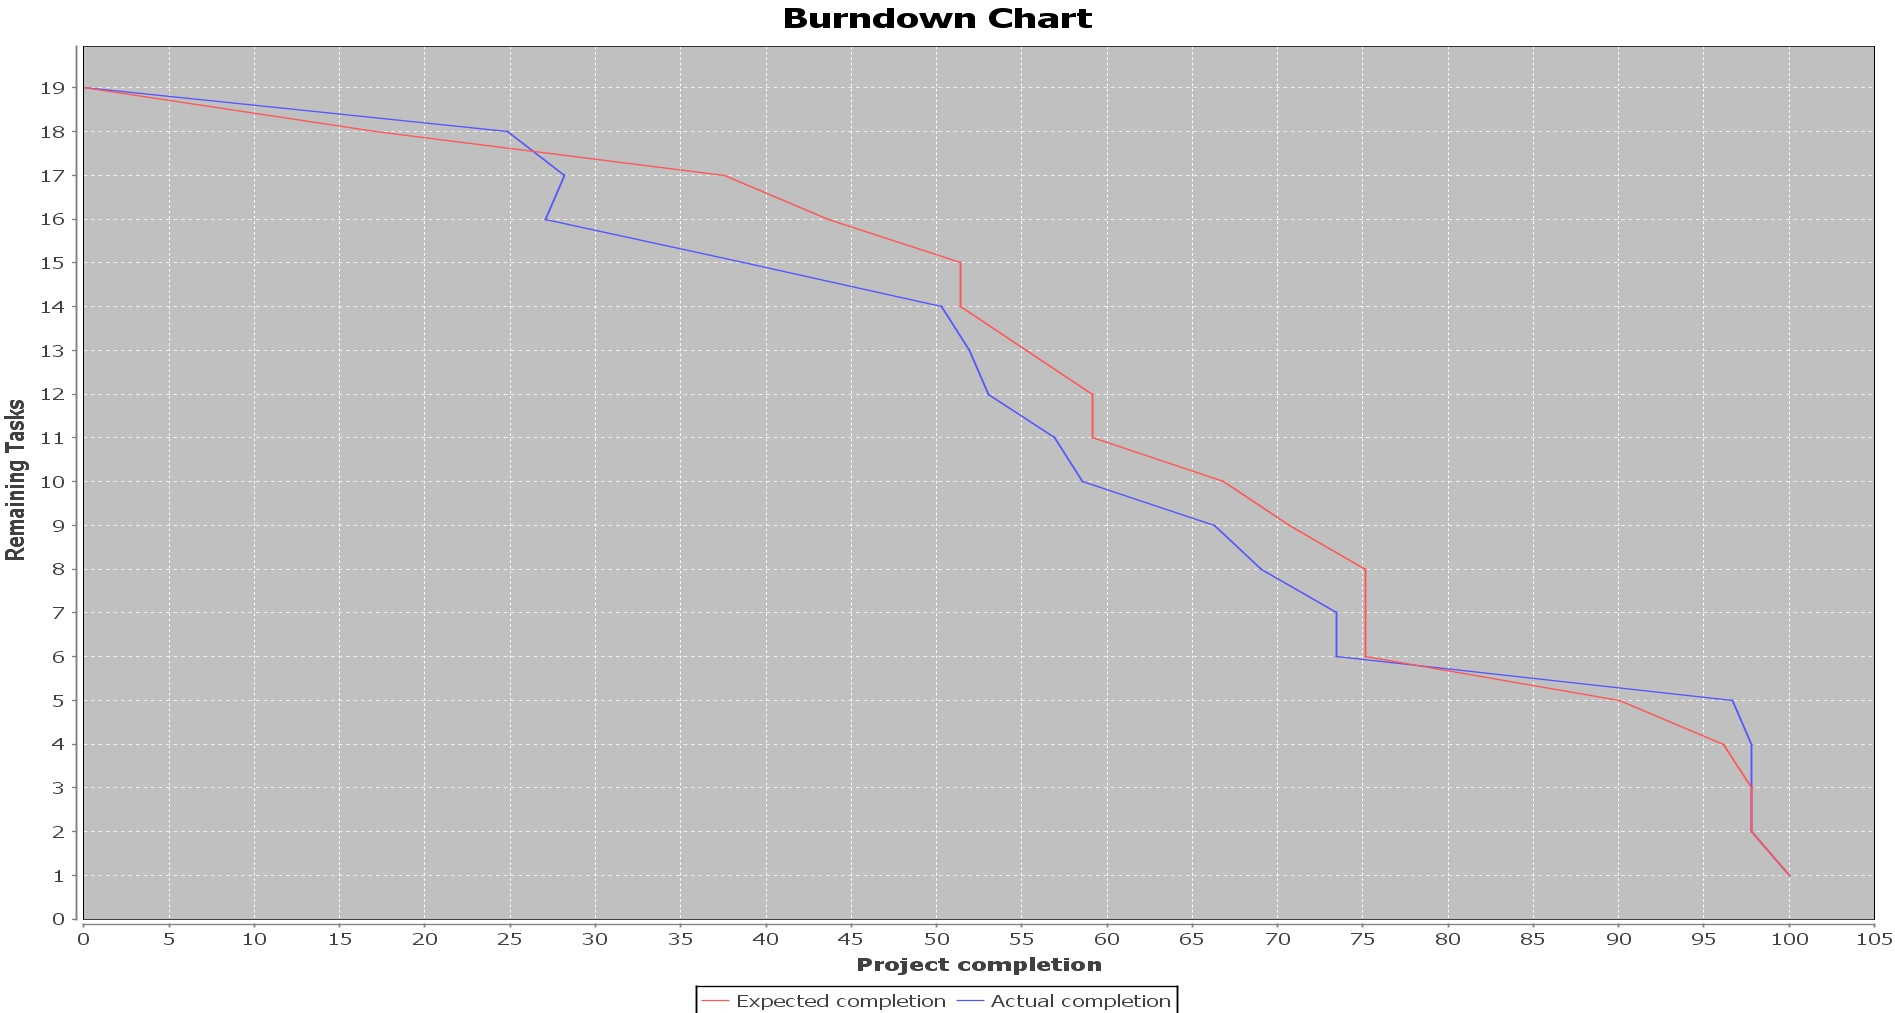
\includegraphics[width=\textwidth,height=120mm]{UML_Diagram/Burndown_Chart.jpg}
			\end{flushleft}
		\end{minipage}
				
		\vspace{0.2in}
	\section*{\colorbox{black}{\makebox[\textwidth-2\fboxsep][l]{\bfseries\color{red} Unimplemented functions }}} \addcontentsline{toc}{section}{Unimplemented functions}
		\vspace{0.1in}
		
		The following functionalities could not be implemented.
		\begin{itemize}
			\item Game port to Android not completed - The controller used for mobs aggression detection is not being created successfully on an Android device, so that it never detects a collision or an overlapping collision box. Thus mob aggression is never trigger to initiate combat between the player and mob.
			\item Loading screen - NiftyGUI has support for a loading screen but when it is required to update the loading progression it does not do it per frame creation. While loading the terrain it does not update the screen which is the highest loading point.
			\item Change password - Password retrieval does exist but no functionality has been added to allow players to change their passwords.
			\item OAuth achievements - Add achievements to the users social media page after killing an amount of zombies.
		\end{itemize}
		
		\vspace{0.2in}
	\section*{\colorbox{black}{\makebox[\textwidth-2\fboxsep][l]{\bfseries\color{red} Main risks and challenges }}} \addcontentsline{toc}{section}{Main risks and challenges}
		\vspace{0.1in}
		
		This project is based on risks and challenges due to the nature of the expected result.
		
		\begin{itemize}
			\item Open-Source pre-requisite:
				\begin{itemize}
					\item Limited the choices we had when selecting technologies.
					\item Increasing the risk factor of using unknown and not highly supported technologies.
					\item Lowered team productivity due to the vast amount of research that is required.
				\end{itemize}
				Solution : \\
				Before project was assigned research was already started to looking what types of game engines are available, the languages they use and what do they provide for competing the project. During the project research was done on each aspect through the community and developers helping us and previous users of the engine.
			\item Unknown technologies:
				\begin{itemize}
					\item An unknown amount of required research on how it is to be used.
					\item Creating working content which is usable incorporation with other existing content.
				\end{itemize}
				Solution: \\
				Creating multiple tests before incorporating it into the game and hours spent on research.
			\item Project scope \& complexity:
				\begin{itemize}
					\item It is our first time creating a game, modelling \& complex back-end server.
					\item Software required to created the game is complex to understand and use.
					\item High scope of project requirements with game, modelling \& back-end.
				\end{itemize}
				Solution: \\
				Sub-diving the project in small manageable pieces, dividing them amongst team members to research \& implement. Prioritizing played a big role in the project we had defined the priorities through the assigned milestone but we are able to switch to any task that at any stage has a higher priority.
			\item Client distance:
				\begin{itemize}
					\item Our client is situated in Durban.
					\item Limited in-person meeting when in Pretoria for work.
					\item Limiting communication to email and video calls biweekly.
				\end{itemize}
				Solution: \\
				Arranging meetings long before hand, proper preparation of what needs to be discussed during meetings. If unknown problems occurs an email could be sent depicting the problem where we ask for help or guidance.
			\item Time management:
				\begin{itemize}
					\item Time schedules between other classes and courses.
					\item Coordination of meetings and group work sessions.
				\end{itemize}
				Solution: \\
				Leave time management to each team member with set dead lines to maintain. Arrange group session with time to prepare that will insure everyone can work together.
		\end{itemize}
		
\end{document}